% 第 18 题多面体结构示意：上下底面为矩形，侧棱延长交于两点；比例不作数学条件。
% 尺寸 a、b、c、d 仅以标签标注在对应棱外侧（源图为示意，不画尺寸箭头）。
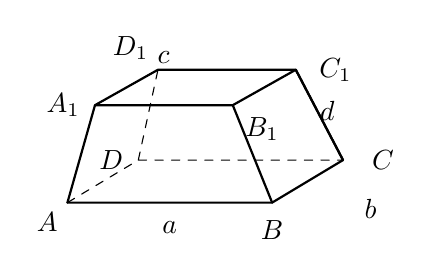
\begin{tikzpicture}[x=1cm,y=.75cm,line cap=round,line join=round]
  \coordinate (A) at (0,0);\coordinate (B) at (2.6,0);\coordinate (C) at (3.5,.72);\coordinate (D) at (.9,.72);
  \coordinate (A1) at (.35,1.65);\coordinate (B1) at (2.1,1.65);\coordinate (C1) at (2.9,2.25);\coordinate (D1) at (1.15,2.25);
  \draw[thick] (A)--(B)--(C)--(C1)--(B1)--(A1)--(D1)--(C1);
  \draw[thick] (A)--(A1) (B)--(B1) (C)--(C1);
  \draw[dashed] (A)--(D) (D)--(C) (D)--(D1);
  % 尺寸标签：置于对应棱外侧，避开棱线与顶点标签
  \node at (1.30,-.42) {$a$};   % 下底面前棱 AB
  \node at (3.85,-.10) {$b$};   % 下底面右棱 BC 外侧
  \node at (1.22,2.46) {$c$};   % 上底面宽 A1B1（顶面后棱之上）
  \node at (3.30,1.55) {$d$};   % 上底面深 B1C1 外侧
  \node[below left] at (A) {$A$};\node[below=3pt] at (B) {$B$};\node[right=7pt] at (C) {$C$};\node[left=2pt] at (D) {$D$};
  \node[left=2pt] at (A1) {$A_1$};\node[below right=1pt] at (B1) {$B_1$};\node[right=5pt] at (C1) {$C_1$};\node[above left] at (D1) {$D_1$};
\end{tikzpicture}
